\documentclass[10pt,a4paper]{article}
\usepackage{amssymb} %mathbb
\usepackage{amsmath} %align
\usepackage{graphicx} %jpg
\usepackage{tikz-cd}
\usepackage[top=1.0cm,bottom=1.3cm,left=1.0cm,right=1.0cm]{geometry}
\usepackage{array,bm}
\newcolumntype{L}{>{$}l<{$}}
\newcolumntype{C}{>{$}c<{$}}
\renewcommand{\arraystretch}{1.2}
\begin{document}

	\normalsize

		Whole mathematics | without categories | is context free. By Vinicius Claudino Ferraz.

		\vspace{3mm}

		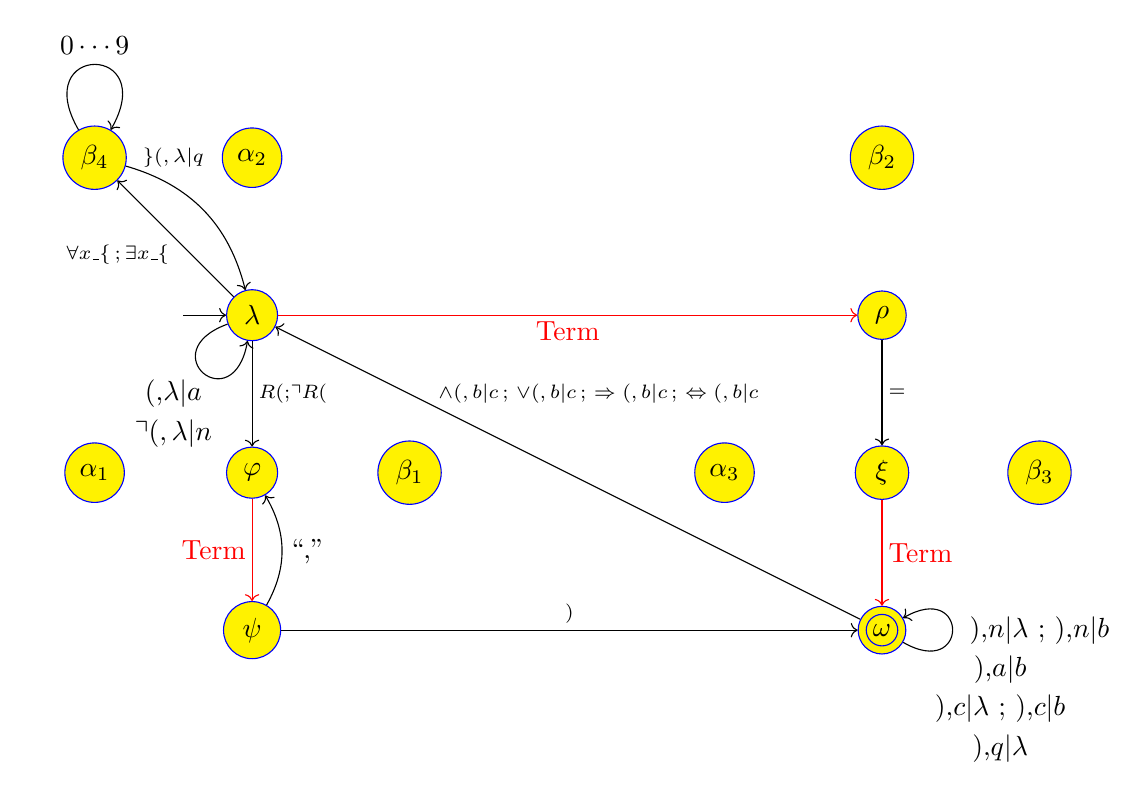
\begin{tikzpicture}
		\node (nada) at (2,0) { };
		\node[draw=blue, circle, fill=yellow] (lambda) at (3,0) {$\lambda$};
		\node (lambdalinha1) at (2,-1) {(,$\lambda|a$};
		\node (lambdalinha2) at (2,-1.5) {$\urcorner(,\lambda|n$};
		\node[font=\scriptsize] (lambdalinha3) at (2, 2) {$\}(,\lambda|q$};
		\draw[->] (lambda) to [in=260,out=200, loop, " "] node { } (lambda);
		\node[font=\scriptsize] (etalinha2) at (7.4, -1) {$\wedge(, b|c\,;\,\vee(, b|c\,;\,\Rightarrow(, b|c\,;\,\Leftrightarrow(, b|c$};
		\node[draw=blue, circle, fill=yellow] (rho) at (11,0) {$\rho$};
		\node[draw=blue, circle, fill=yellow] (xi) at (11,-2) {$\xi$};
		\node[draw=blue, circle, fill=yellow] (omega) at (11,-4) {$\omega$};
		\node (omegalinha1) at (13, -4) {),$n|\lambda$ ; ),$n|b$};
		\node (omegalinha2) at (12.5, -4.5) {),$a|b$};
		\node (omegalinha3) at (12.5, -5) {),$c|\lambda$ ; ),$c|b$};
		\node (omegalinha3) at (12.5, -5.5) {),$q|\lambda$};
		\draw[blue] (11,-4) circle (0.2);
		\draw[->] (omega) to [in=30,out=330, loop, " "] node { } (omega);
		\node[draw=blue, circle, fill=yellow] (varphi) at (3,-2) {$\varphi$};
		\node[draw=blue, circle, fill=yellow] (alpha1) at (1,-2) {$\alpha_1$};
		\node[draw=blue, circle, fill=yellow] (c1) at (5,-2) {$\beta_1$};
		\node[draw=blue, circle, fill=yellow] (psi) at (3,-4) {$\psi$};
		\node (psilinha) at (3.7, -3) {``,"};
		\node[draw=blue, circle, fill=yellow] (c4) at (1,2) {$\beta_4$};
		\node[draw=blue, circle, fill=yellow] (alpha2) at (3,2) {$\alpha_2$};
		\node[draw=blue, circle, fill=yellow] (c2) at (11,2) {$\beta_2$};
		\node[draw=blue, circle, fill=yellow] (c3) at (13,-2) {$\beta_3$};
		\node[draw=blue, circle, fill=yellow] (alpha3) at (9,-2) {$\alpha_3$};
		\draw[->] (c4) to [in=60,out=120, loop, "$0\cdots 9$"] node { } (c4);
		\draw[->, bend right] (psi) to node { } (varphi);
		\draw[->, bend left] (c4) to node { } (lambda);
		\path[commutative diagrams/.cd, every arrow, every label]
		(nada) edge node { } (lambda)
		(lambda) edge[red] node[swap] {Term} (rho) edge node {$R( ; \urcorner R($} (varphi) edge node {$\forall x\_\{\,;\,\exists x \_\{$} (c4)
		(rho) edge node {$=$} (xi)
		(xi) edge[red] node {Term} (omega)
		(omega) edge node { } (lambda)
		(varphi) edge[red] node[swap] {Term} (psi)
		(psi) edge node {$)$} (omega);
		\end{tikzpicture}

		\vspace{3mm}

		$F \rightarrow$ Term $=$ Term

		$F \rightarrow R\_\{N\}(P)$

		$F \rightarrow \urcorner R\_\{N\}(P)$

		$P \rightarrow$ Term

		$P \rightarrow P, P$

		$\lambda \rightarrow F$

		$\lambda \rightarrow_aX_{ab}Y_cX_c$

		$X \rightarrow (F)$

		$X \rightarrow_aX_{ab}Y_cX_c$

		$F \rightarrow \urcorner (_nF)_n$

		$F \rightarrow \forall x\_\{N\} (_qF)_q$

		$F \rightarrow \exists x\_\{N\} (_qF)_q$

		$N \rightarrow NN$

		$N \rightarrow 0|1|2|3|4|5|6|7|8|9$

		$Y \rightarrow \wedge|\vee|\Rightarrow|\Leftrightarrow$

		\vspace{3mm}

		Now we're going to define a Term.

		\vspace{3mm}

		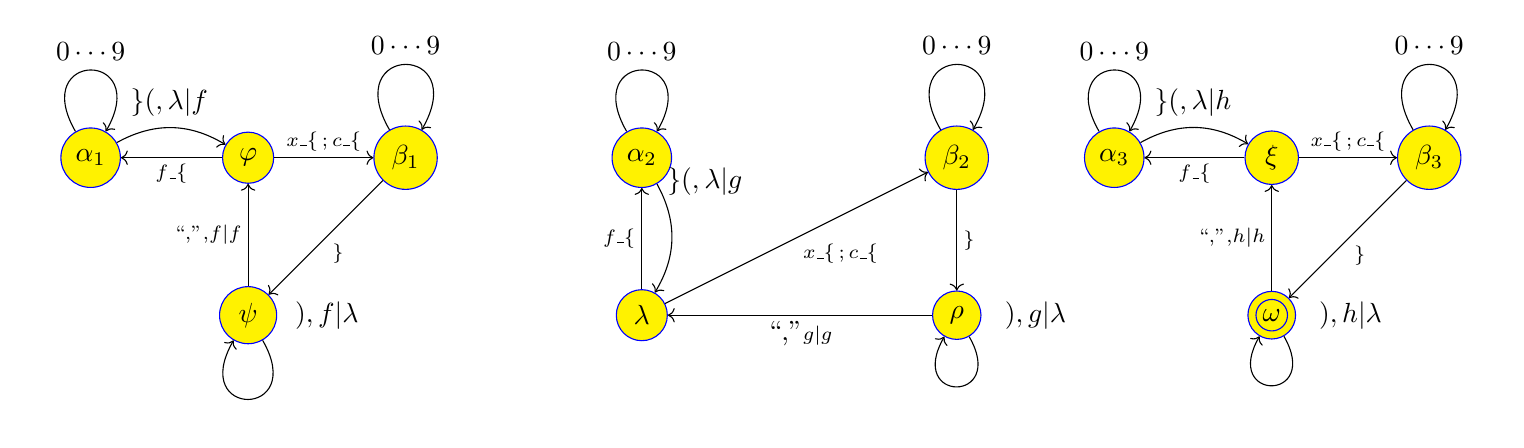
\begin{tikzpicture}
		\node[draw=blue, circle, fill=yellow] (alpha) at (0,-2) {$\alpha_1$};
		\node (alphalinha) at (1, -1.3) {$\}(,\lambda|f$};
		\draw[->] (alpha) to [in=60,out=120, loop, "$0\cdots9$"] node { } (alpha);
		\node[draw=blue, circle, fill=yellow] (varphi) at (2,-2) {$\varphi$};
		\node[draw=blue, circle, fill=yellow] (c) at (4,-2) {$\beta_1$};
		\draw[->] (c) to [in=60,out=120, loop, "$0\cdots9$"] node { } (c);
		\node[draw=blue, circle, fill=yellow] (psi) at (2,-4) {$\psi$};
		\node (psilinha) at (3, -4) {$),f|\lambda$};
		\draw[->] (psi) to [in=240,out=300, loop, " "] node { } (psi);
		\draw[->, bend left] (alpha) to node { } (varphi);
		\path[commutative diagrams/.cd, every arrow, every label]
		(varphi) edge node {$f\_\{$} (alpha) edge node {$x\_\{\,;\,c\_\{$} (c)
		(c) edge node {$\}$} (psi)
		(psi) edge node {$``,", f|f$} (varphi);
		\node[draw=blue, circle, fill=yellow] (alpha) at (7,-2) {$\alpha_2$};
		\node (alphalinha) at (7.8, -2.3) {$\}(,\lambda|g$};
		\draw[->] (alpha) to [in=60,out=120, loop, "$0\cdots9$"] node { } (alpha);
		\node[draw=blue, circle, fill=yellow] (varphi) at (7,-4) {$\lambda$};
		\node[draw=blue, circle, fill=yellow] (c) at (11,-2) {$\beta_2$};
		\draw[->] (c) to [in=60,out=120, loop, "$0\cdots9$"] node { } (c);
		\node[draw=blue, circle, fill=yellow] (psi) at (11,-4) {$\rho$};
		\node (psilinha1) at (12, -4) {$), g|\lambda$};
		\draw[->] (psi) to [in=240,out=300, loop, " "] node { } (psi);
		\draw[->, bend left] (alpha) to node { } (varphi);
		\path[commutative diagrams/.cd, every arrow, every label]
		(varphi) edge node {$f\_\{$} (alpha) edge node[swap] {$x\_\{\,;\,c\_\{$} (c)
		(c) edge node {$\}$} (psi)
		(psi) edge node {``,"$g|g$} (varphi);
		\node[draw=blue, circle, fill=yellow] (alpha) at (13,-2) {$\alpha_3$};
		\node (alphalinha) at (14, -1.3) {$\}(,\lambda|h$};
		\draw[->] (alpha) to [in=60,out=120, loop, "$0\cdots9$"] node { } (alpha);
		\node[draw=blue, circle, fill=yellow] (varphi) at (15,-2) {$\xi$};
		\node[draw=blue, circle, fill=yellow] (c) at (17,-2) {$\beta_3$};
		\draw[->] (c) to [in=60,out=120, loop, "$0\cdots9$"] node { } (c);
		\node[draw=blue, circle, fill=yellow] (psi) at (15,-4) {$\omega$};
		\draw[blue] (15,-4) circle (0.2);
		\node (psilinha1) at (16, -4) {$),h|\lambda$};
		\draw[->] (psi) to [in=240,out=300, loop, " "] node { } (psi);
		\draw[->, bend left] (alpha) to node { } (varphi);
		\path[commutative diagrams/.cd, every arrow, every label]
		(varphi) edge node {$f\_\{$} (alpha) edge node {$x\_\{\,;\,c\_\{$} (c)
		(c) edge node {$\}$} (psi)
		(psi) edge node {$``,", h|h$} (varphi);
		\end{tikzpicture}

		\vspace{3mm}

		Term $\rightarrow x\_\{N\}$

		Term $\rightarrow c\_\{N\}$

		Term $\rightarrow f\_\{N\}(_fP)_f$

		Term $\rightarrow f\_\{N\}(_gP)_g$

		Term $\rightarrow f\_\{N\}(_hP)_h$

		\vspace{120mm}

		Now we're going to post some figures for dummies.

		\begin{center}
		\includegraphics[scale=.5]{21}
		\end{center}

		\begin{center}
		\includegraphics[scale=.5]{31}
		\end{center}

		\begin{center}
		\includegraphics[scale=.5]{32}
		\end{center}

		For instance:

		\begin{center}
		\includegraphics[scale=1]{exemplos}
		\end{center}

		\vspace{120mm}

		Conclusion:

		\vspace{3mm}

		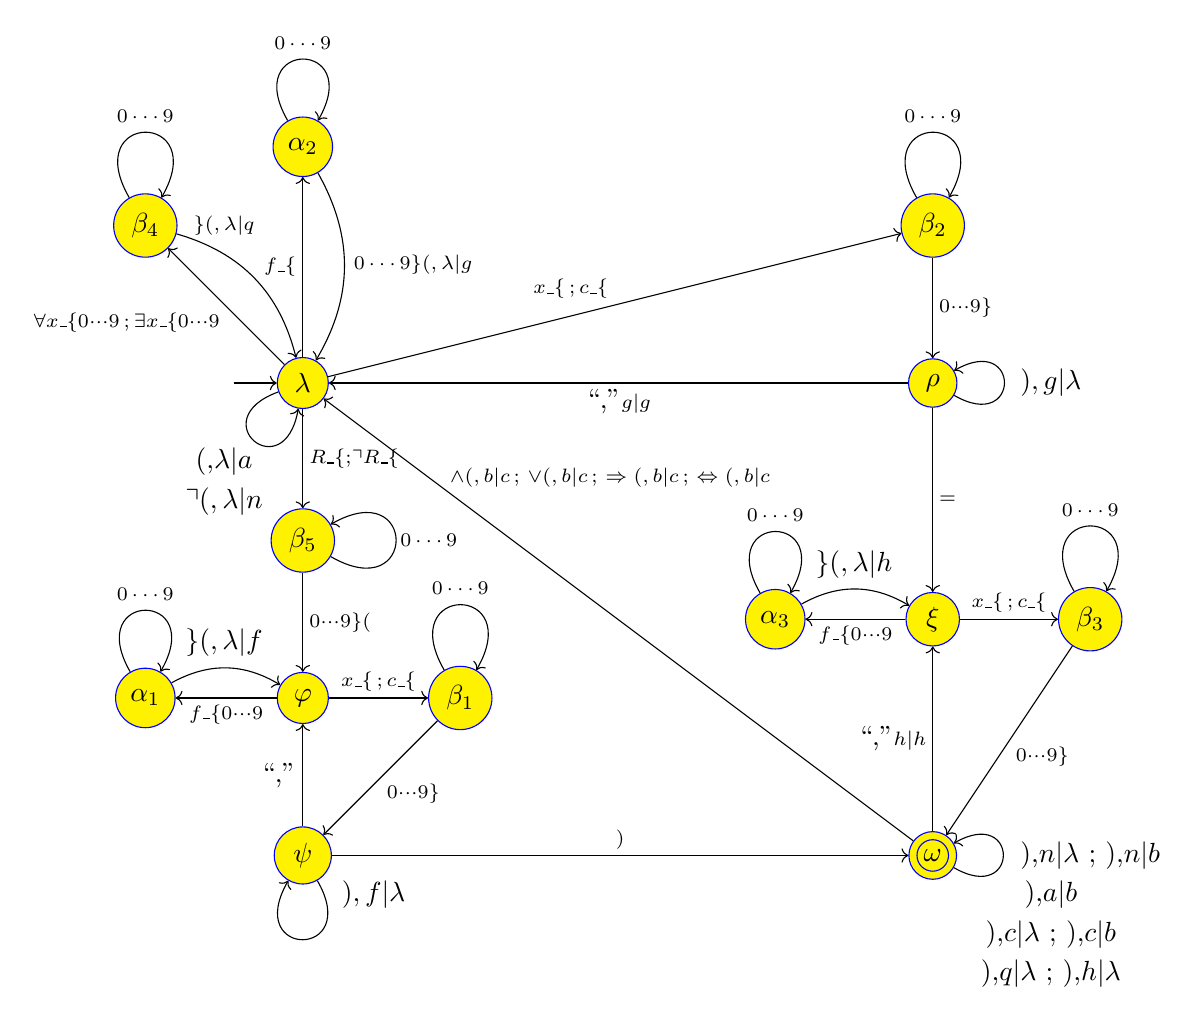
\begin{tikzpicture}
		\node (nada) at (2,0) { };
		\node[draw=blue, circle, fill=yellow] (lambda) at (3,0) {$\lambda$};
		\node (lambdalinha1) at (2,-1) {(,$\lambda|a$};
		\node (lambdalinha2) at (2,-1.5) {$\urcorner(,\lambda|n$};
		\node[font=\scriptsize] (lambdalinha2B) at (4.6,-2) {$0\cdots 9$};
		\node[font=\scriptsize] (lambdalinha3) at (4.4, 1.5) {$0\cdots 9\}(,\lambda|g$};
		\node[font=\scriptsize] (lambdalinha4) at (2, 2) {$\}(,\lambda|q$};
		\draw[->] (lambda) to [in=260,out=200, loop, " "] node { } (lambda);
		\node[font=\scriptsize] (lambdalinha5) at (6.9, -1.2) {$\wedge(, b|c\,;\,\vee(, b|c\,;\,\Rightarrow(, b|c\,;\,\Leftrightarrow(, b|c$};
		\node (lambdalinha8) at (2, -3.3) {$\}(,\lambda|f$};
		\node (lambdalinha9) at (10, -2.3) {$\}(,\lambda|h$};
		\node[draw=blue, circle, fill=yellow] (rho) at (11,0) {$\rho$};
		\node[draw=blue, circle, fill=yellow] (xi) at (11,-3) {$\xi$};
		\node[draw=blue, circle, fill=yellow] (omega) at (11,-6) {$\omega$};
		\node (omegalinha1) at (13, -6) {),$n|\lambda$ ; ),$n|b$};
		\node (omegalinha2) at (12.5, -6.5) {),$a|b$};
		\node (omegalinha3) at (12.5, -7) {),$c|\lambda$ ; ),$c|b$};
		\node (omegalinha4) at (12.5, -7.5) {),$q|\lambda$ ; ),$h|\lambda$};
		\node (omegalinha5) at (12.5, 0) {$),g|\lambda$};
		\draw[blue] (11,-6) circle (0.2);
		\draw[->] (rho) to [in=30,out=330, loop, " "] node { } (rho);
		\draw[->] (omega) to [in=30,out=330, loop, " "] node { } (omega);
		\node[draw=blue, circle, fill=yellow] (c5) at (3,-2) {$\beta_5$};
		\draw[->, font=\scriptsize] (c5) to [in=30,out=330, loop, " "] node { } (c5);
		\node[draw=blue, circle, fill=yellow] (varphi) at (3,-4) {$\varphi$};
		\node[draw=blue, circle, fill=yellow] (alpha1) at (1,-4) {$\alpha_1$};
		\node[draw=blue, circle, fill=yellow] (c1) at (5,-4) {$\beta_1$};
		\node[draw=blue, circle, fill=yellow] (psi) at (3,-6) {$\psi$};
		\node (psilinha) at (3.9, -6.5) {$),f|\lambda$};
		\node[draw=blue, circle, fill=yellow] (c4) at (1,2) {$\beta_4$};
		\node[draw=blue, circle, fill=yellow] (alpha2) at (3,3) {$\alpha_2$};
		\node[draw=blue, circle, fill=yellow] (c2) at (11,2) {$\beta_2$};
		\node[draw=blue, circle, fill=yellow] (c3) at (13,-3) {$\beta_3$};
		\node[draw=blue, circle, fill=yellow] (alpha3) at (9,-3) {$\alpha_3$};
		\draw[->, font=\scriptsize] (c1) to [in=60,out=120, loop, "$0\cdots 9$"] node { } (c1);
		\draw[->, font=\scriptsize] (c2) to [in=60,out=120, loop, "$0\cdots 9$"] node { } (c2);
		\draw[->, font=\scriptsize] (c3) to [in=60,out=120, loop, "$0\cdots 9$"] node { } (c3);
		\draw[->, font=\scriptsize] (c4) to [in=60,out=120, loop, "$0\cdots 9$"] node { } (c4);
		\draw[->, font=\scriptsize] (alpha1) to [in=60,out=120, loop, "$0\cdots 9$"] node { } (alpha1);
		\draw[->, font=\scriptsize] (alpha2) to [in=60,out=120, loop, "$0\cdots 9$"] node { } (alpha2);
		\draw[->, font=\scriptsize] (alpha3) to [in=60,out=120, loop, "$0\cdots 9$"] node { } (alpha3);
		\draw[->] (psi) to [in=240,out=300, loop, " "] node { } (psi);
		\draw[->, bend left] (c4) to node { } (lambda);
		\draw[->, bend left] (alpha2) to node { } (lambda);
		\draw[->, bend left] (alpha1) to node { } (varphi);
		\draw[->, bend left] (alpha3) to node { } (xi);
		\path[commutative diagrams/.cd, every arrow, every label]
		(nada) edge node { } (lambda)
		(lambda) edge node {$R\_\{ ; \urcorner R\_\{$} (c5) edge node {$\forall x\_\{0\cdots 9\,;\,\exists x \_\{0\cdots 9$} (c4)	edge node {$f\_\{$} (alpha2) edge node {$x\_\{\,;\,c\_\{$} (c2)
		(rho) edge node {$=$} (xi) edge node {``,"$g|g$} (lambda)
		(xi) edge node {$f\_\{0\cdots 9$} (alpha3) edge node {$x\_\{\,;\,c\_\{$} (c3)
		(omega) edge node { } (lambda) edge node {``,"$h|h$} (xi)
		(varphi) edge node {$f\_\{0\cdots 9$} (alpha1) edge node {$x\_\{\,;\,c\_\{$} (c1)
		(c1) edge node {$0\cdots 9\}$} (psi)
		(c2) edge node {$0\cdots 9\}$} (rho)
		(c3) edge node {$0\cdots 9\}$} (omega)
		(c5) edge node {$0\cdots 9\}($} (varphi)
		(psi) edge node {$)$} (omega) edge node {``,"} (varphi);
		\end{tikzpicture}

\end{document}
